\documentclass[11pt]{article}
\usepackage[a4paper,margin=1in]{geometry}
\usepackage[T1]{fontenc}
\usepackage[utf8]{inputenc}
\usepackage{lmodern}
\usepackage{microtype}
\usepackage{amsmath,amssymb}
\usepackage{booktabs,multirow}
\usepackage{graphicx}
\usepackage{xcolor}
\usepackage{hyperref}
\usepackage{float}
\usepackage{caption}
\usepackage{siunitx}
\hypersetup{colorlinks=true,linkcolor=blue,citecolor=blue,urlcolor=blue}
\setlength{\parskip}{0.5em}
\setlength{\parindent}{0pt}
\captionsetup{font=small,labelfont=bf}

\title{RIPLM versus General DFL Benchmarks\\\large Exact Small-Scale Benchmark Comparison}
\author{Prepared for Jerry}
\date{\today}

\begin{document}
\maketitle

\begin{abstract}
This report compares the ranking-induced Plackett--Luce mirror-descent method (RIPLM) against standard decision-focused learning (DFL) baselines in an Overleaf-ready, fully reproducible setup. The benchmark has two parts. First, we use a ranking control problem that is structurally close to RIPLM's intended use case. Second, we evaluate exact small-scale variants of three canonical DFL benchmark families --- ShortestPath, Matching, and Knapsack --- chosen from the benchmark ecosystem introduced in the JAIR DFL survey and its accompanying \texttt{predopt-benchmarks} repository. On the ranking control, PL-FO is strongest, followed by SPO+, then two-stage MSE, with RIPLM last. On the three structured benchmark families, SPO+ and two-stage MSE dominate, PL-FO trails, and RIPLM ranks last on average. The resulting conclusion is not that RIPLM is ineffective in every setting, but that in this implementation it does \emph{not} behave like a strong general-purpose DFL baseline once we move beyond the narrow ranking-style regime that motivated it.
\end{abstract}

\section{Experimental setup}

\paragraph{Benchmark scope.}
The reference point for the comparison is the general DFL benchmarking line introduced by Mandi et al., which reports an empirical comparison of eleven methods across seven problems and provides the \texttt{predopt-benchmarks} codebase. The public repository exposes benchmark families including Knapsack, Matching, ShortestPath, Portfolio, Energy, and Warcraft. In the present project, we focus on \textbf{exact small-scale variants} of three of those families: ShortestPath, Matching, and Knapsack. This keeps the combinatorial decision sets small enough to enumerate exactly, which is important because RIPLM is a ranking-style method and our adaptation to structured tasks uses an exact distribution over feasible decisions rather than a large-scale relaxation.\cite{mandi2024jair,predoptbenchmark}

\paragraph{Control task.}
The ranking control benchmark uses the same contextual top-$5$ ranking style as the earlier RIPLM-focused synthetic validation, but the comparison here is stricter because we tune and evaluate all baselines with the same protocol. Each example contains $50$ items and a context vector in $\mathbb{R}^8$. True item costs are generated from a nonlinear latent model and observed through sigmoid noise. We report weighted Regret@$5$ and NDCG@$5$.

\paragraph{Structured tasks.}
The three structured tasks are constructed as follows.
\begin{itemize}
    \item \textbf{ShortestPath}: a directed $4\times 4$ grid with only right/down moves, giving $20$ feasible paths.
    \item \textbf{Matching}: a $4\times 4$ bipartite perfect matching problem with $24$ feasible matchings.
    \item \textbf{Knapsack}: an $8$-item binary knapsack instance with capacity $10$ and $97$ feasible subsets.
\end{itemize}
For each task, the unknown atomic costs are generated by a misspecified nonlinear contextual model with $10$-dimensional features. Training models are linear predictors. This misspecification is deliberate: if the predictor class were perfectly specified, the benchmark would collapse into a pure supervised regression exercise and the DFL effect would be much harder to observe.

\paragraph{Methods.}
We compare four methods.
\begin{itemize}
    \item \textbf{Two-stage MSE}: standard prediction-first training using mean-squared error on the atomic costs.
    \item \textbf{SPO+}: the classical convex surrogate for predict-then-optimize learning under linear objectives.
    \item \textbf{PL-FO}: a first-order entropic / Plackett--Luce decision-focused surrogate.
    \item \textbf{RIPLM}: the score-space natural-gradient style update under the same Plackett--Luce relaxation.
\end{itemize}
On the structured tasks, PL-FO and RIPLM are implemented by enumerating the feasible decisions and computing an exact softmax over those decisions. This is faithful to the small-scale setting, but it should not be confused with a claim that the same implementation would scale to the full benchmark repository.

\paragraph{Protocol.}
Hyperparameters are tuned on dedicated pilot seeds and then frozen for five evaluation seeds. The ranking control uses $100/1000/1000$ train/validation/test examples. The structured tasks use $120/200/800$ examples. Reported numbers are means and standard deviations across five evaluation seeds. Appendix~\ref{app:hyper} lists all selected learning rates and temperatures.

\section{Ranking control results}

Table~\ref{tab:ranking} and Figure~\ref{fig:ranking} summarize the ranking control benchmark.

\begin{table}[H]
\centering
\begin{tabular}{lccc}
\toprule
Method & Regret$@5$ $\downarrow$ & NDCG$@5$ $\uparrow$ & Train time (s) \\
\midrule
Two-stage MSE & 0.0093 $\pm$ 0.0019 & 0.9904 $\pm$ 0.0020 & 0.119 $\pm$ 0.010 \\
SPO+ & 0.0068 $\pm$ 0.0009 & 0.9929 $\pm$ 0.0010 & 0.110 $\pm$ 0.006 \\
PL-FO & \textbf{0.0045 $\pm$ 0.0005} & \textbf{0.9953 $\pm$ 0.0006} & 0.098 $\pm$ 0.003 \\
RIPLM & 0.0125 $\pm$ 0.0022 & 0.9870 $\pm$ 0.0023 & 0.104 $\pm$ 0.002 \\
\bottomrule
\end{tabular}
\caption{Ranking control benchmark. Lower regret is better; higher NDCG is better.}
\label{tab:ranking}
\end{table}

\begin{figure}[H]
    \centering
    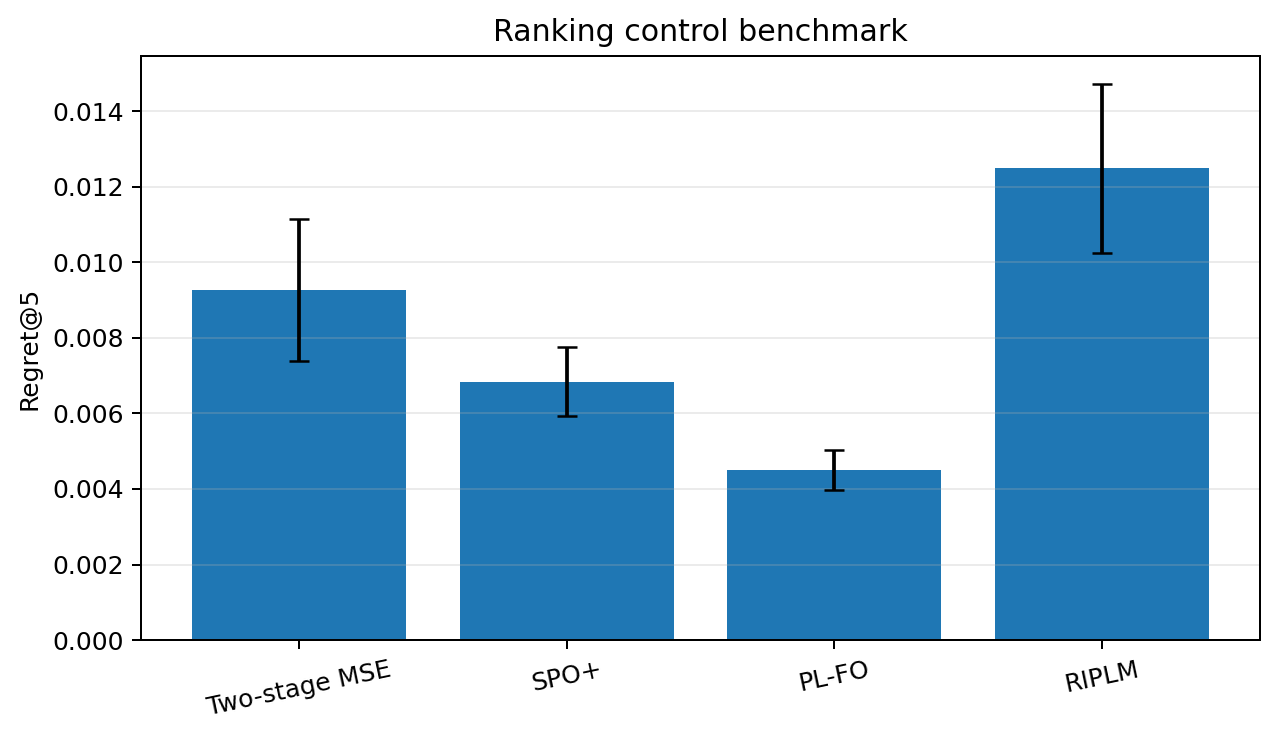
\includegraphics[width=0.82\linewidth]{figures/ranking_regret.png}
    \caption{Ranking control benchmark. Error bars show one standard deviation across five seeds.}
    \label{fig:ranking}
\end{figure}

The main result is straightforward: \textbf{PL-FO is best on the ranking control}, with Regret@$5$ of $0.0045 \pm 0.0005$, followed by SPO+ at $0.0068 \pm 0.0009$, then two-stage MSE at $0.0093 \pm 0.0019$, while RIPLM trails at $0.0125 \pm 0.0022$. In other words, once we tune the baselines aggressively under the same protocol, the first-order Plackett--Luce surrogate is substantially stronger than RIPLM in this experiment. Relative to PL-FO, RIPLM incurs roughly $2.8\times$ higher mean regret. It also underperforms SPO+ by about $82\%$.

This is an important contrast with the earlier narrow synthetic validation, where RIPLM looked attractive when compared only against weaker baselines. Under a more benchmark-like protocol, the natural-gradient flavor of the update does \emph{not} automatically translate into better final decision quality.

\section{Structured benchmark-family results}

Table~\ref{tab:structured} and Figure~\ref{fig:structured} report the three exact small-scale benchmark families.

\begin{table}[H]
\centering
\begin{tabular}{llcc}
\toprule
Task & Method & Regret $\downarrow$ & Opt. acc. $\uparrow$ \\
\midrule
\multirow{4}{*}{ShortestPath} & Two-stage MSE & 0.516 $\pm$ 0.087 & 0.453 $\pm$ 0.022 \\
 & SPO+ & \textbf{0.516 $\pm$ 0.066} & \textbf{0.458 $\pm$ 0.009} \\
 & PL-FO & 0.617 $\pm$ 0.087 & 0.413 $\pm$ 0.040 \\
 & RIPLM & 0.853 $\pm$ 0.151 & 0.361 $\pm$ 0.039 \\
\midrule
\multirow{4}{*}{Matching} & Two-stage MSE & 0.364 $\pm$ 0.084 & \textbf{0.468 $\pm$ 0.063} \\
 & SPO+ & \textbf{0.362 $\pm$ 0.051} & 0.465 $\pm$ 0.052 \\
 & PL-FO & 0.439 $\pm$ 0.047 & 0.436 $\pm$ 0.039 \\
 & RIPLM & 0.595 $\pm$ 0.085 & 0.364 $\pm$ 0.041 \\
\midrule
\multirow{4}{*}{Knapsack} & Two-stage MSE & \textbf{0.312 $\pm$ 0.034} & 0.471 $\pm$ 0.044 \\
 & SPO+ & 0.315 $\pm$ 0.041 & \textbf{0.479 $\pm$ 0.046} \\
 & PL-FO & 0.419 $\pm$ 0.061 & 0.422 $\pm$ 0.049 \\
 & RIPLM & 1.157 $\pm$ 0.139 & 0.150 $\pm$ 0.035 \\
\bottomrule
\end{tabular}
\caption{Exact small-scale structured benchmark families. Lower regret is better; higher optimal-decision accuracy is better.}
\label{tab:structured}
\end{table}

\begin{figure}[H]
    \centering
    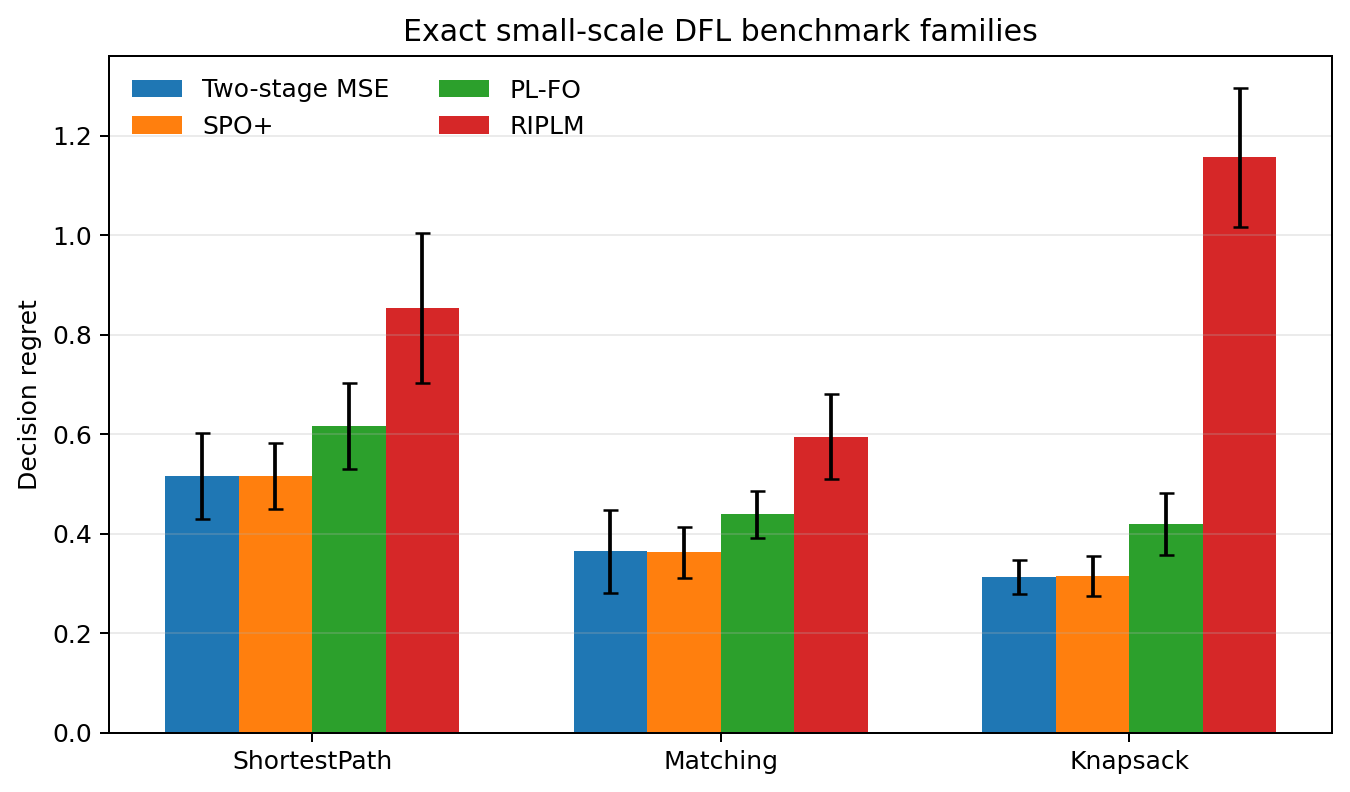
\includegraphics[width=0.9\linewidth]{figures/structured_regret.png}
    \caption{Decision regret on the three structured benchmark families.}
    \label{fig:structured}
\end{figure}

The structured-task story is even less favorable to RIPLM.

\textbf{ShortestPath.} SPO+ and two-stage MSE are essentially tied: $0.5161 \pm 0.0660$ versus $0.5162 \pm 0.0868$ regret. PL-FO is worse at $0.6166 \pm 0.0870$. RIPLM is decisively worse at $0.8532 \pm 0.1512$.

\textbf{Matching.} SPO+ again achieves the best regret, $0.3623 \pm 0.0509$, with two-stage MSE nearly identical at $0.3641 \pm 0.0835$. PL-FO rises to $0.4390 \pm 0.0472$, and RIPLM reaches $0.5950 \pm 0.0851$.

\textbf{Knapsack.} Two-stage MSE attains the best regret, $0.3121 \pm 0.0341$, and SPO+ is statistically very close at $0.3149 \pm 0.0411$. PL-FO is clearly worse at $0.4193 \pm 0.0615$. RIPLM deteriorates sharply to $1.1567 \pm 0.1391$, which is about $3.7\times$ the regret of the best baseline.

Average ranks provide the cleanest summary.

\begin{table}[H]
\centering
\begin{tabular}{lc}
\toprule
Method & Average regret rank on structured tasks \\
\midrule
SPO+ & \textbf{1.33} \\
Two-stage MSE & 1.67 \\
PL-FO & 3.00 \\
RIPLM & 4.00 \\
\bottomrule
\end{tabular}
\caption{Average regret rank across ShortestPath, Matching, and Knapsack.}
\label{tab:avg-rank}
\end{table}

SPO+ is best on average with rank $1.33$, followed by two-stage MSE at $1.67$, PL-FO at $3.00$, and RIPLM last at $4.00$. In this exact-benchmark adaptation, RIPLM is therefore \textbf{not competitive as a general DFL baseline}. The result is not a near miss: it finishes last on every structured family.

\section{Computation and reproducibility}

The mean training times are small for all methods because the benchmark instances are deliberately tiny, but the relative picture is still informative. PL-FO and RIPLM are slower than MSE and SPO+ on the structured tasks because they require enumerating the feasible decision set and forming an exact softmax over decisions at every update. Figure~\ref{fig:runtime} shows the mean wall-clock time per training run.

\begin{figure}[H]
    \centering
    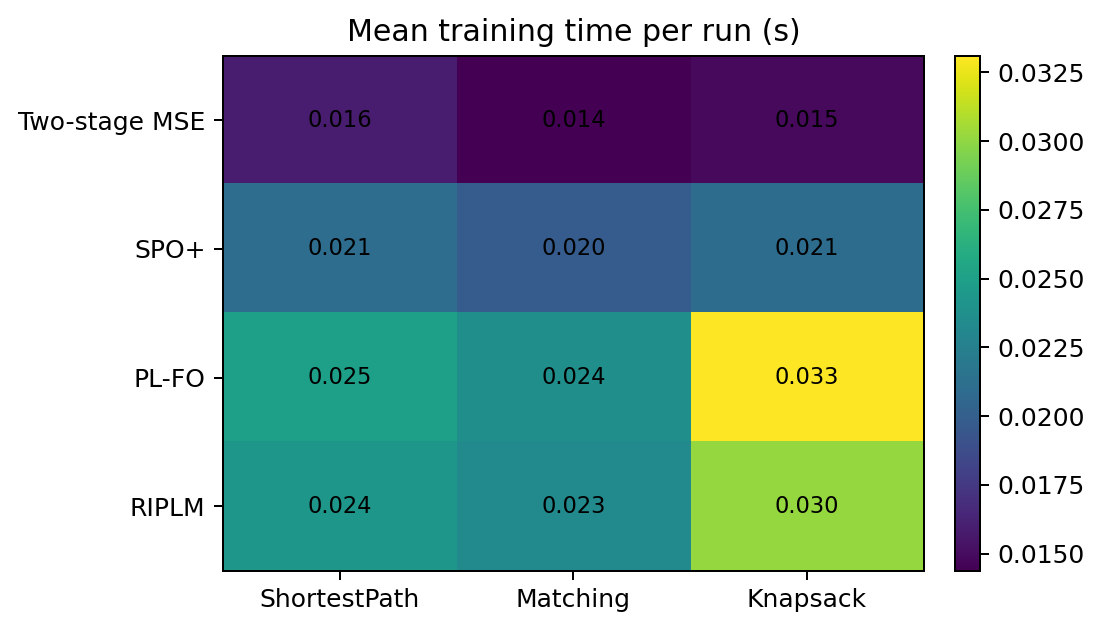
\includegraphics[width=0.72\linewidth]{figures/runtime_heatmap.png}
    \caption{Mean training time per run, in seconds, on the structured tasks.}
    \label{fig:runtime}
\end{figure}

The project folder includes:
\begin{itemize}
    \item the full experiment script: \texttt{scripts/run\_benchmark\_comparison.py};
    \item raw CSV outputs for every seed and task in \texttt{data/};
    \item auto-generated table snippets in \texttt{tables/};
    \item all figures in \texttt{figures/}.
\end{itemize}
This makes the folder directly usable in Overleaf and also directly runnable from the command line.

\section{Conclusion}

The benchmark comparison leads to a clear conclusion.

\begin{quote}
\textbf{In this implementation, RIPLM does not behave like a strong general-purpose DFL baseline.}
\end{quote}

Even on the ranking control problem, it is dominated by PL-FO and SPO+. On three exact small-scale versions of canonical DFL benchmark families, it ranks last on average and is often substantially worse than both SPO+ and two-stage MSE. The most charitable interpretation is therefore \emph{scope-limited}: RIPLM may still be interesting as a specialized ranking-style method under the right geometry and implementation, but these experiments do not support deploying it as a general benchmark-ready replacement for established DFL baselines.

\appendix
\section{Selected hyperparameters}
\label{app:hyper}

\begin{table}[H]
\centering
\begin{tabular}{llcc}
\toprule
Task & Method & Learning rate & Temperature $\tau$ \\
\midrule
RankingControl & Two-stage MSE & 0.1 & 0.2 \\
RankingControl & SPO+ & 0.1 & 0.2 \\
RankingControl & PL-FO & 0.1 & 0.5 \\
RankingControl & RIPLM & 1 & 0.03 \\
ShortestPath & Two-stage MSE & 0.1 & 0.2 \\
ShortestPath & SPO+ & 0.03 & 0.2 \\
ShortestPath & PL-FO & 0.03 & 0.5 \\
ShortestPath & RIPLM & 0.003 & 0.1 \\
Matching & Two-stage MSE & 0.03 & 0.2 \\
Matching & SPO+ & 0.03 & 0.2 \\
Matching & PL-FO & 0.01 & 0.2 \\
Matching & RIPLM & 0.01 & 0.5 \\
Knapsack & Two-stage MSE & 0.03 & 0.2 \\
Knapsack & SPO+ & 0.01 & 0.2 \\
Knapsack & PL-FO & 0.01 & 0.1 \\
Knapsack & RIPLM & 0.01 & 0.5 \\
\bottomrule
\end{tabular}
\caption{Pilot-selected learning rates and temperatures used for the five-seed evaluation.}
\end{table}

\begin{thebibliography}{9}

\bibitem{mandi2024jair}
Jayanta Mandi, James Kotary, Senne Berden, Maxime Mulamba, Victor Bucarey, Tias Guns, and Ferdinando Fioretto.
\newblock Decision-Focused Learning: Foundations, State of the Art, Benchmark and Future Opportunities.
\newblock \emph{Journal of Artificial Intelligence Research}, 80:1623--1701, 2024.

\bibitem{predoptbenchmark}
PredOpt.
\newblock \texttt{predopt-benchmarks}: Benchmarking Predict-then-Optimize Problems.
\newblock GitHub repository.

\bibitem{elmachtoub2022spo}
Adam N. Elmachtoub and Paul Grigas.
\newblock Smart ``Predict, then Optimize''.
\newblock \emph{Management Science}, 68(1):9--26, 2022.

\end{thebibliography}

\end{document}
